\documentclass[12pt, twoside]{article}
\usepackage{jmlr2e}
\usepackage[utf8x]{inputenc} % Включаем поддержку UTF8  
\usepackage[russian]{babel}  % Включаем пакет для поддержки русского языка  
\usepackage[]{algorithmic}
\usepackage{graphicx}
\usepackage{multicol}
\usepackage{caption}
\usepackage{subfig}
\newcommand{\hdir}{.}
\newtheorem{statement}{Утверждение}
\usepackage{graphicx} % more modern
\usepackage{subcaption} 
\usepackage{multirow}
\usepackage{mathtools}
\usepackage{relsize}
\usepackage{url}
\usepackage{nicefrac}
\usepackage{xspace}
\usepackage{algorithm}
\usepackage{algorithmic}
\usepackage{multicol}
\usepackage{float}
\usepackage{bbm}




\usepackage[dvipsnames]{xcolor}
\usepackage{pifont}
\newcommand{\cmark}{{\color{PineGreen}\ding{51}}}%
\newcommand{\xmark}{{\color{BrickRed}\ding{55}}}%

\usepackage[utf8]{inputenc} % allow utf-8 input
\usepackage[T1]{fontenc}    % use 8-bit T1 fonts
\usepackage{hyperref}       % hyperlinks
\usepackage{url}            % simple URL typesetting

\usepackage{nicefrac}       % compact symbols for 1/2, etc.
\usepackage{microtype}      % microtypography 
 
 % style
% \usepackage{fullpage}
\usepackage{layout}
\usepackage{multirow}
% \usepackage{cases}

% ams
\usepackage{amsfonts}
\usepackage{amsmath}
\usepackage{amssymb} % NOT COMATIBLE WITH svjour3

% shaded theorems
\usepackage{mdframed} 
\usepackage{thmtools}

\usepackage[font=normalsize, labelfont=bf]{caption}
%\newtheoremstyle{selfdefined}
%{12pt}% Space above
%{12pt}% Space below
%{}% Body font \itshape =italian style 
%{}% Indent amount
%{\bfseries}% Theorem head font
%{}% Punctuation after theorem heading
%{\newline}% Space after theorem heading, 0.5em => in gleicher zeile weiter
%{}% Theorem head spec (can be left empty, meaning ‘normal’)




% captions
% \usepackage{caption}
% \usepackage{subcaption}


% graphics
% \usepackage[dvips]{graphicx}
% \usepackage{colordvi,epsfig}
\usepackage{color}
\usepackage{graphicx}
\graphicspath{{plots/}}

\usepackage{xcolor}

% algorithms
\usepackage{algorithm}
%\usepackage{algorithmic}
%\usepackage[noend]{algpseudocode}
\usepackage{verbatim}
\usepackage[algo2e]{algorithm2e} 


\usepackage[symbol]{footmisc}
\renewcommand{\thefootnote}{\fnsymbol{footnote}}

% various
% \usepackage{url}
%\usepackage[cp1250]{inputenc}
%\usepackage[T1]{fontenc}
%\usepackage{calligra}
%\usepackage[slovak]{babel}
%\usepackage{charter}


% What is this?
% \PassOptionsToPackage{normalem}{ulem}
% \usepackage{ulem}
%% Change tracking with ulem

\def\<{\left\langle}
\def\>{\right\rangle}
% \def\[{\left[}
%\def\]{\right]}
\def\({\left(}
\def\){\right)}


\def\supp{{\rm supp}}
\newcommand{\sphere}{\mathbb{S}}

\newcommand{\BR}{\text{BR}}
\newcommand{\NC}{\cC_{\rm nat}}
\newcommand{\NCd}{\cC_{\rm nat}^{\rm det}}
\newcommand{\Qint}{\cC_{\rm int}}
\newcommand{\ND}{\cD_{\rm nat}^{p,s}}
\newcommand{\GD}{\cD_{\rm gen}^{\cC ,p,s}}
\newcommand{\SD}{\cD_{\rm sta}^{p,s}}
\newcommand{\SDs}[1]{\cD_{\rm sta}^{p,#1}}
%\newcommand{\floor}[1]{\lfloor#1\rfloor}
%\newcommand{\ceil}[1]{\lceil#1\rceil	}


%\newcommand{\BR}{\text{BR}}
%\newcommand{\NC}{\cC_{\rm nat}}
%\newcommand{\Qint}{\cC_{\rm int}}
%\newcommand{\ND}{\cD_{\rm nat}^{p,s}}
%\newcommand{\GD}{\cD_{\rm gen}^{\cC ,p,s}}
%\newcommand{\SD}{\cD_{\rm sta}^{p,s}}
%\newcommand{\SDs}[1]{\cD_{\rm sta}^{p,#1}}


\newcommand{\smartparagraph}[1]{\noindent {\bf #1}}

\newcommand\tagthis{\addtocounter{equation}{1}\tag{\theequation}}

\newcommand{\reals}{\mathbb{R}}
\newcommand{\note}[1]{\textcolor{red}{#1}}
\newcommand{\ip}[2]{\left\langle #1, #2\right\rangle}
\newcommand{\nlsum}{\sum\nolimits}

\DeclareMathOperator{\Ocal}{\mathcal{O}} 
\DeclareMathOperator{\sign}{sign} 

%%%%%%%%%%%%%%%%%%%%%%%%%
%%%%%% BIBLIOGRAPHY
%%%%%%%%%%%%%%%%%%%%%%%%%

%\usepackage[maxbibnames=99, maxcitenames=10,doi=false,isbn=false,url=false,backend=bibtex]{biblatex}
%%\bibliography{SDA.bib}
%\newcommand{\Ref}[1]{../ref/#1}
%%\input{\Ref{biblatex_journal_def}}

%%% Basic sets

% caligraphic
\newcommand{\cA}{{\cal A}}
\newcommand{\cB}{{\cal B}}
\newcommand{\cC}{{\cal C}}
\newcommand{\cD}{{\cal D}}
\newcommand{\cE}{{\cal E}}
\newcommand{\cF}{{\cal F}}
\newcommand{\cG}{{\cal G}}
\newcommand{\cH}{{\cal H}}
\newcommand{\cJ}{{\cal J}}
\newcommand{\cK}{{\cal K}}
\newcommand{\cL}{{\cal L}}
\newcommand{\cM}{{\cal M}}
\newcommand{\cN}{{\cal N}}
\newcommand{\cO}{{\cal O}}
\newcommand{\cP}{{\cal P}}
\newcommand{\cQ}{{\cal Q}}
\newcommand{\cR}{{\cal R}}
\newcommand{\cS}{{\cal S}}
\newcommand{\cT}{{\cal T}}
\newcommand{\cU}{{\cal U}}
\newcommand{\cV}{{\cal V}}
\newcommand{\cX}{{\cal X}}
\newcommand{\cY}{{\cal Y}}
\newcommand{\cW}{{\cal W}}
\newcommand{\cZ}{{\cal Z}}

%
\newcommand{\R}{\mathbb{R}} % reals
\newcommand{\C}{\mathbb{C}}
\newcommand{\Z}{\mathbb{Z}}
\newcommand{\I}{\mathbb{I}}
\newcommand{\B}{\mathbb{B}}
\newcommand{\N}{\mathbb{N}} % Naturals
\newcommand{\U}{\mathbb{U}}


% bold
\newcommand{\bA}{{\bf A}}
\newcommand{\bB}{{\bf B}}
\newcommand{\bC}{{\bf C}}
\newcommand{\bE}{{\bf E}}
\newcommand{\bI}{{\bf I}}
\newcommand{\bS}{{\bf S}}
\newcommand{\bZ}{{\bf Z}}

% red matrices
%\newcommand{\mA}{{\color{red}\bf A}}
%\newcommand{\mB}{{\color{red}\bf B}}
%\newcommand{\mC}{{\color{red}\bf C}}
%\newcommand{\mE}{{\color{red}\bf E}}
%\newcommand{\mF}{{\color{red}\bf F}}
%\newcommand{\mG}{{\color{red}\bf G}}
%\newcommand{\mH}{{\color{red}\bf H}}
%\newcommand{\mI}{{\color{red}\bf I}}
%\newcommand{\mJ}{{\color{red}\bf J}}
%\newcommand{\mK}{{\color{red}\bf K}}
%\newcommand{\mL}{{\color{red}\bf L}}
%\newcommand{\mM}{{\color{red}\bf M}}
%\newcommand{\mN}{{\color{red}\bf N}}
%\newcommand{\mO}{{\color{red}\bf O}}
%\newcommand{\mP}{{\color{red}\bf P}}
%\newcommand{\mQ}{{\color{red}\bf Q}}
%\newcommand{\mR}{{\color{red}\bf R}}
%\newcommand{\mS}{{\color{red}\bf S}}
%\newcommand{\mT}{{\color{red}\bf T}}
%\newcommand{\mU}{{\color{red}\bf U}}
%\newcommand{\mV}{{\color{red}\bf V}}
%\newcommand{\mW}{{\color{red}\bf W}}
%\newcommand{\mX}{{\color{red}\bf X}}
%\newcommand{\mY}{{\color{red}\bf Y}}
%\newcommand{\mZ}{{\color{red}\bf Z}}

% matrices
\newcommand{\mA}{{\bf A}}
\newcommand{\mB}{{\bf B}}
\newcommand{\mC}{{\bf C}}
\newcommand{\mD}{{\bf D}}

\newcommand{\mE}{{\bf E}}
\newcommand{\mF}{{\bf F}}
\newcommand{\mG}{{\bf G}}
\newcommand{\mH}{{\bf H}}
\newcommand{\mI}{{\bf I}}
\newcommand{\mJ}{{\bf J}}
\newcommand{\mK}{{\bf K}}
\newcommand{\mL}{{\bf L}}
\newcommand{\mM}{{\bf M}}
\newcommand{\mN}{{\bf N}}
\newcommand{\mO}{{\bf O}}
\newcommand{\mP}{{\bf P}}
\newcommand{\mQ}{{\bf Q}}
\newcommand{\mR}{{\bf R}}
\newcommand{\mS}{{\bf S}}
\newcommand{\mT}{{\bf T}}
\newcommand{\mU}{{\bf U}}
\newcommand{\mV}{{\bf V}}
\newcommand{\mW}{{\bf W}}
\newcommand{\mX}{{\bf X}}
\newcommand{\mY}{{\bf Y}}
\newcommand{\mZ}{{\bf Z}}
\newcommand{\mLambda}{{\bf \Lambda}}

\newcommand{\zeros}{{\bf 0}}
\newcommand{\ones}{{\bf 1}}


%\newcommand{\red}[1]{{\color{red} #1}}
%\newcommand{\blank}[1]{\{#1\}}

%\providecolor{added}{rgb}{0,0,1}
%\providecolor{deleted}{rgb}{1,0,0}
%\newcommand{\added}[1]{{\color{added}{}#1}}
%\newcommand{\deleted}[1]{{\color{deleted}\sout{#1}}}
%\newcommand{\ignore}[1]{}

\newcommand{\mcnote}[1]{\todo[inline]{\textbf{Marco: }#1}}

\newcommand{\YY}{\gamma}
\newcommand{\XX}{\omega}


\newcommand{\Sam}{S}  


% basic
%\newcommand{\eqdef}{\overset{\text{def}}{=}} 
\newcommand{\eqdef}{\coloneqq}

\newcommand{\st}{\;:\;} % such that
\newcommand{\ve}[2]{\langle #1 ,  #2 \rangle} % inner
\newcommand{\lin}[1]{\langle #1 \rangle} % inner product
\newcommand{\dotprod}[1]{\left< #1\right>} % product
\newcommand{\norm}[1]{\left\| #1 \right\|_2}      % norm 
\newcommand{\onenorm}[1]{\left\| #1 \right\|_1}      % norm 
\newcommand{\twonorm}[1]{\left\| #1 \right\|_2}      % norm 
\newcommand{\threenorm}[1]{\left\| #1 \right\|_3}      % norm 

\newcommand{\Elias}{\mathrm{Elias}}
\newcommand{\Comp}{\mathrm{Code}}


% sets
\DeclareMathOperator{\card}{card}       % cardinality of a set
\DeclareMathOperator{\diam}{diam}       % diameter of a set
\DeclareMathOperator{\MVEE}{MVEE}       % minim volume enclosing ellipsoid of a set
\DeclareMathOperator{\vol}{vol}         % volume of a set 

% statistical
%\DeclareMathOperator{\Exp}{\mathbf{E}} % expectation
\DeclareMathOperator{\Cov}{Cov}         % covariance
\DeclareMathOperator{\Var}{Var}         % variance
\DeclareMathOperator{\Corr}{Corr}       % correlation
\DeclareMathOperator{\Prob}{Prob}
% \newcommand{\Prob}{\mathbf{Prob}}


% functions and operators
\DeclareMathOperator{\signum}{sign}     % signum/sign of a scalar
\DeclareMathOperator{\dom}{dom}         % domain
\DeclareMathOperator{\epi}{epi}         % epigraph
% \DeclareMathOperator{\Ker}{null}        % nullspace/kernel
\DeclareMathOperator{\nullspace}{null}  % nullpsace
% \DeclareMathOperator{\range}{range}     % range
% \DeclareMathOperator{\Image}{Im}        % image
\DeclareMathOperator{\argmin}{argmin}        % argmin
\DeclareMathOperator{\prox}{prox}       % proximal operator      

% topology
\DeclareMathOperator{\interior}{int}    % interior
\DeclareMathOperator{\ri}{rint}         % relative interior
\DeclareMathOperator{\rint}{rint}       % relative interior
\DeclareMathOperator{\bdry}{bdry}       % boundary
\DeclareMathOperator{\cl}{cl}           % closure

% vectors, matrices
\DeclareMathOperator{\linspan}{span}
\DeclareMathOperator{\linspace}{linspace}
\DeclareMathOperator{\cone}{cone}
\DeclareMathOperator{\traceOp}{tr}           % trace
\DeclareMathOperator{\rank}{rank}       % rank
\DeclareMathOperator{\conv}{conv}       % convex hull
%\DeclareMathOperator{\Diag}{Diag}       % Diag(v) = diagonal matrix with v_i on the diagonal
\DeclareMathOperator{\diag}{diag}       % diag(D) = the diagonal vector of matrix D
\DeclareMathOperator{\Arg}{Arg}         % Argument
\DeclarePairedDelimiter\ceil{\lceil}{\rceil}
\DeclarePairedDelimiter\floor{\lfloor}{\rfloor}

% operators with parentheses
%\newcommand{\normB}[1]{\lVert#1\rVert}
%\newcommand{\dotprodB}[1]{\left< #1\right>}
%\newcommand{\trB}[1]{\mathbf{Tr}\left( #1\right)}
\newcommand{\Diag}[1]{\mathbf{Diag}\left( #1\right)}
\providecommand{\kernel}[1]{{\rm Null}\left( #1\right)}
%\providecommand{\rankB}[1]{\mathbf{Rank}\left( #1\right)}
\providecommand{\range}[1]{{\rm Range}\left( #1\right)}
\providecommand{\span}[1]{{\rm Span}\left\{ #1\right\}}
\providecommand{\trace}[1]{{\rm Trace}\left( #1\right)}
%\providecommand{\projB}[2]{\mbox{proj}_{#1}^{#2}}

\newcommand{\expSB}[2]{{ \mathbf{E}}_{#1}\left[#2\right] } % expectation with subscript
\newcommand{\Exp}[1]{{{\rm E}}\left[#1\right] }    % expectation
\newcommand{\ExpC}[1]{{{\rm E_C}}\left[#1\right] }
\newcommand{\Expg}[1]{{{\rm E_{\nabla}}}\left[#1\right] }
%\newcommand{\inner}[1]{\langle#1\rangle}
\newcommand{\E}[1]{{\rm E}\left[#1\right] } 
\newcommand{\Esimple}{{\rm E}} 
\newcommand{\EE}[2]{{\rm E}_{#1}\left[#2\right] } 
\newcommand{\ED}[1]{{\rm E}_{S\sim \cD}\left[#1\right] }
\newcommand{\abs}[1]{| #1 |} 



\newtheorem{assumption}{Assumption}

\begin{document}


\title{Применение операторов сжатия в задачах распределенной оптимизации}

\author{\name Касюк Вадим  \email kasiuk.va@phystech.edu\\}

\maketitle

\begin{abstract}% <- trailing '%' for backward compatibility of .sty file

В работе предлагаются 3 новых смещенных оператора сжатия. Рассматривается их применения в задачах распределенной оптимизации. Получены теоретические гарантии сходимости методов с этими операторами в случаях одного и нескольких устройств, оценена асимптотика сходимости. Проведены численные эксперименты, показывающие превосходство предложенных операторов над стандартными: Top-k, Rand-K, для случая 1 устройства на примере классических алгоритмов машинного обучения и нейросетей.

\end{abstract}

\begin{keywords}
  Compression operators, biased compressors, distributed learning, linear convergence
\end{keywords}


\section{Введение}
Применение методов распределенной оптимизации сейчас активно используется в задачах, которые невозможно эффективно решить на одном вычислительном устройстве из-за ограничений памяти или вычислительных мощностей. Кроме того, потребность в более совершенных способах вычислений только увеличивается с каждым годом.

Важную роль в распределенной оптимизации занимают методы, которые пытаются сократить расходы на общение между устройствами в процессе вычислений. Особый интерес представляют операторы сжатия, которые уменьшают количество передаваемой информации. 

Операторы сжатия делятся на 2 группы: смещенные и несмещенные. Несмещенные давно и хорошо изученные операторы, которые на практике демонстрируют меньшую производительность, в сравнении с смешенными. Несмотря на это, лишь сравнительно недавно появилась математическая теория, описывающая вторых. 

\subsection{Распределенная оптимизация}

Решается задача оптимизации :
\begin{equation} 
\label{general_problem}
\underset{x\in R^d}{min} \ f(x) := \frac{1}{n} \sum_{i=1}^n f_i(x),
\end{equation}
где $x \in R^d$ - пространство признаков размерности $d$, $n$ - количество устройст/узлов, $f_i(x) : R^d \rightarrow R$ - потери, которые получает модель на устройстве под номером $i$. Часто функция потерь имеем вид : 

\begin{equation*}f_i(x) = E_{\xi \sim P_i} [f_{\xi}(x)],\end{equation*} где $P_i$ - это распределение тренировочных данных на устройстве $i$. То, как данные распределяются между работниками оказывает большое влияние на процесс обучения.


В данной работе рассматривается случай централизованного типа : 

\begin{enumerate} 
\item  Имеется $n$ работников, каждый производит вычисления градиента функции $f_i(x)$( или стохастического градиента) парралельно с другими.

\item  Устройства посылают посчитанный градиент на главное устройство - сервер

\item  Сервер обрабатывает посчитанный градиент, делает шаг градиентного спуска и передает новую информацию каждому устройству, для выполнения новый вычислений. И затем процесс повторяется.
 
\end{enumerate}
Большие временные потери приходятся на общение между сервером и устройствами. Именно для их уменьшения используется операторы сжатия.

\subsection{Базовое решение}
Базовым решением задачи (\ref{general_problem}) является обычный градиентный спуск (GD), который имеет вид :
\begin{equation}
    \label{GD}
    x^{k+1} = x^k - \frac{\eta^k}{n} \sum_{i=1}^n \nabla f_i(x^k)
\end{equation}
где, $\eta^k > 0$ - темп обучения или размер шага. Базовое решение уже подвергалось улучшению: использование ускорение(Нестеров), использование моментума(Метод тяжелого шарика)(Тут вообще общие ускоренные методы), уменьшение количества обмена информации с сервером, посредством выполения нескольких шагов локально(Надо найти источник), а также уменьшения размеров передаваемой информации за счет использования операторов сжатия(Тут можно вставить Безноса и его предшественника)(Здесь уже другие подходы к распределенным вычислениям).

\subsection{Связанные работы}
Ранее была проведена обширная работа, связанная со сжатием сообщений, в основном сосредоточенная
на несмещенном сжатии \cite{alistarh2017qsgd}, поскольку его гораздо легче анализировать. В частности, было
показано \cite{gorbunov2019unifiedtheorysgdvariance}, что как классический метод с несмещенным сжатием \cite{alistarh2017qsgd}, так и более продвинутые
модификации \cite{mishchenko2023distributedlearningcompressedgradient} могут рассматриваться как специальные версии SGD. Впоследствии результаты
\cite{gorbunov2019unifiedtheorysgdvariance} для сильно выпуклых задач были перенесены на выпуклые \cite{li2020unifiedanalysisstochasticgradient} и невыпуклые целевые функции
\cite{vogels2020powersgdpracticallowrankgradient}. В то же время работы, касающиеся смещенных сжатий, показывают более сильные резульаты.


Получены эмпирические результаты, но с ограниченным анализом или без него \cite{pmlr-v80-wu18d}. Было предпринято несколько попыток решить эту проблему, например, "проведен анализ для квадратичных чисел в распределенной среде".Был проведен анализ для momentum SGD с определенным смещенным сжатием, но с необоснованными предположениями, т.е. с ограниченной нормой градиента и памятью. Первый результат, который позволил получить линейную скорость сходимости при смещенном сжатии, был получен с помощью \cite{shi2024globalmomentumcompressionsparse}, но только для одного узла и в
предположении об ограниченной норме градиента, которое позже было преодолено с помощью \cite{karimireddy2019errorfeedbackfixessignsgd}.


Использование смещенного сжатия для распределенного обучения
улучшило теоретические гарантии. Недавно был разработан новый вариант механизма обратной связи по ошибкам.Введено в \cite{fatkhullin2021ef21bellswhistles}, показывающее улучшенные показатели для распределенных невыпуклых задач.

Более всего автор опирается на работу \cite{beznosikov2024biasedcompressiondistributedlearning}, где автор вводит 3 семейства смещенных операторов, анализирует их свойства, получает гарантии сходимости для них и в общем развивает идею : "Смещенные операторы вычислительно эффективнее несмещенных".
\subsection{Нотация и определения}

Мы используем  $\lin{ x,y } \eqdef \sum_{i=1}^d x_i y_i$ для обозначения стандартного скалярного произведения 2-ух векторов  $x,y\in\R^d$, где $x_i$ обозначает $i$-ую компонетну $x$ в стандартном базисе $\R^d$. Скалярное произведение индуцирует $\ell_2$-норму в  $\R^d$ следующим образом : $\twonorm{x} \eqdef\sqrt{\lin{ x, x }}$.  Также $\ell_p$-норма определяется как $\|x\|_p \eqdef (\sum_{i=1}^d|x_i|^p)^{\nicefrac{1}{p}}$ для $p\in(1,\infty)$.
С помощью $\Exp{\cdot}$, мы обозначамаем математическое ожидание.
Дифференцируемая функция $f:\R^d\to \R$ называется $L$-гладкой, если :
$$f(y) \leq f(x) + \lin{\nabla f(x), y-x} + \frac{L}{2}\norm{y-x}^2,  \qquad \forall x,y\in \R^d.$$
Функция $f:\R^d\to \R$ $\mu$-сильно выпуклая, если :
$$f(y) \geq f(x) + \lin{\nabla f(x), y-x} + \frac{\mu}{2} \norm{y-x}^2, \qquad \forall x,y\in \R^d.$$ 

\section{Смещенные операторы}
Под операторами сжатия мы подразумеваем (возможно рандомизированное) отображение $\cC\colon\R^d\to\R^d$ с некоторыми требованиями.
Как правило, в литературе рассматриваются {\em несмещенные} операторы сжатия $\cC$ с ограниченным вторым моментом, т.е. :

\begin{definition}
Пусть $\zeta \geq 1$. Тогда  $\cC\in \mathbb{U}(\zeta)$ если $\cC$ явлется несмещенным (то есть, $\Exp{\cC(x)}=x$ для любых $x$) и втором момент ограничен \footnote{\eqref{eq:unbiased} Что также может быть переписанное в виде $\Exp{ \twonorm{\cC(x) -x }^2 } \leq (\zeta-1)  \twonorm{x}^2 $.}
\begin{equation}\label{eq:unbiased}
 \Exp{ \twonorm{\cC(x)}^2 } \leq \zeta  \twonorm{x}^2, \qquad \forall x\in\R^d \,.
\end{equation} 

\end{definition}

\subsection{3 класса смещенных операторов}
\begin{definition}\label{def:comp_I}
Будем говорить, что  $\cC\in \mathbb{B}^1(\alpha,\beta)$ для некторых $\alpha,\beta>0$ если
\begin{equation} \label{eq:alpha-beta} \alpha \twonorm{x}^2 \leq \Exp{ \twonorm{\cC(x)}^2 } \leq \beta  \langle \Exp{\cC(x)},x \rangle, \qquad \forall x\in\R^d \; .
\end{equation}
\end{definition}

И в статье(Безносикова вставить ссылку) доказывается, что \eqref{eq:alpha-beta} влечет за собой $\Exp{ \twonorm{\cC(x)}^2 } \leq \beta^2 \twonorm{x}^2$. 

Во втором классе мы требуем, чтобы скалярное произведение между несжатым $x$  и сжатым $\cC(x)$ вектором мажорировало квадраты норм этих векторов Берется математическое ожидание от сжатого вектора, поскольку оператор может быть рандомизированным.

\begin{definition}\label{def:comp_II}
Будем говорить, что $\cC\in \mathbb{B}^2(\gamma,\beta)$ для некторых $\gamma,\beta>0$ если
\begin{equation} \label{eq:alpha-betaII}
\max\left\{ \gamma \twonorm{x}^2 , \tfrac{1}{\beta} \Exp{\twonorm{\cC(x)}^2}\right\} \leq \lin{\Exp{\cC(x)},x } \qquad \forall x\in\R^d \,.
\end{equation}
\end{definition}


Наконец, в третьем классе мы требуем, чтобы ошибка сжатия  $\twonorm{\cC(x) - x}^2$ была строго меньше чем 2-норма $\twonorm{x}^2$ входного вектора $x$ в среднем.

\begin{definition}\label{def:comp_III}
Будем говорить, что $\cC\in \mathbb{B}^3(\delta)$ для некоторого $\delta>0$ если
\begin{equation}\label{eq:biasedIII}
\Exp{ \twonorm{\cC(x) - x}^2 } \leq \left(1 - \frac{1}{\delta}\right)\twonorm{x}^2, \qquad  \forall x\in\R^d \; .
\end{equation}
\end{definition}
\subsection{Примеры смещенных и несмещенных операторов}

\begin{itemize}
\item[(a)] Для $k \in [d]\eqdef \{1,\dots,d\}$,  {\bf несмещенный случайный  (aka Rand-$k$) сжимающий} определяется как :
\begin{equation}\label{ex:ur-sparse}
\cC(x) \eqdef \frac{d}{k}\sum \limits_{i\in S}x_ie_i,
\end{equation}
где $S\subseteq [d]$ подмножество индексов размера $k$ выбранных равновероятно, и $e_1,\dots,e_d$ стандартные базисные вектора $\R^d$.

\begin{lemma}\label{lem-ex:ur-sparse}
Rand-$k$ оператор (\ref{ex:ur-sparse}) принадлежит $U (\tfrac{d}{k})$.
\end{lemma}


\item[(b)] Пусть $S\subseteq [d]$ случайное множество индексов, с вектором вероятности получения элементов $p\eqdef (p_1,\dots,p_d)$, где  $p_i \eqdef \Prob(i\in S)>0$ для любых $i$ . Определим {\bf случайный смещенный сжимающий} оператор как :
\begin{equation}\label{ex:br-sparse}
 \cC(x) \eqdef \sum \limits_{i\in S} x_i e_i.
\end{equation}

\begin{lemma}\label{lem-ex:br-sparse}
Пусть $q \eqdef \min_i p_i$, тогда случайный смещенный сжимающий оператор (\ref{ex:br-sparse}) принадлежит $\mathbb{B}^1(q, 1)$, $\mathbb{B}^2(q, 1)$, $\mathbb{B}^3(\nicefrac{1}{q})$.
\end{lemma}

\item[(c)] {\bf Адаптивный случайный смещенный оператор} определяется, как :
\begin{equation}\label{ex:ar-sparse}
\cC(x) \eqdef x_i e_i \quad \text{ с вероятностью } \quad \frac{|x_i|}{\onenorm{x}}.
\end{equation}

\begin{lemma}\label{lem-ex:ar-sparse}
Адаптивный случайный смещенный оператор (\ref{ex:ar-sparse}) принадлежит $\mathbb{B}^1(\frac{1}{d},1)$, $\mathbb{B}^2(\frac{1}{d},1)$, $\mathbb{B}^3(d)$.
\end{lemma}

\item[(d)] {\bf Жадный (aka Top-$k$) сжимающий} оператор определяется, как :
\begin{equation}\label{ex:top-sparse}
\cC(x) \eqdef \sum \limits_{i=d-k+1}^d x_{(i)} e_{(i)},
\end{equation}
где координаты упорядочены по их абсолютным значениям $\abs{x_{(1)}} \leq \abs{x_{(2)}} \leq \cdots \leq \abs{x_{(d)}}$.

\begin{lemma}\label{lem-ex:top-sparse}
Top-$k$ сжимающий оператор (\ref{ex:top-sparse}) принадлежит $\mathbb{B}^1(\frac{k}{d},1)$, $\mathbb{B}^2(\frac{k}{d},1)$, и $\mathbb{B}^3(\frac{d}{k})$.
\end{lemma}

\end{itemize}

Доказательство лемм представлено в \cite{beznosikov2024biasedcompressiondistributedlearning}
\section{Градиентный спуск с компрессией}
Теперь поставим задачу оптимизаци, которую будем решать с помощью градиентного спуска с сжатием(CGD - compressed gredient descent). Пускай решается задача:
\begin{equation}
    \label{unconstrayed_problem}
    \underset{x\in R^d}{min} \ f(x)
\end{equation}, где $f : R^d \rightarrow R$, $L$ - гладкая и $\mu$-сильно-выпуклая, методом :
\begin{equation}
    \label{CGD}
    x^{k+1} = x^k - \eta C(\nabla f(x))
\end{equation}, где $C : R^d \rightarrow R^d$ - оператор сжатия и $\eta > 0$ - темп обучения.

\subsection{Новые операторы сжатия}
Предлагается рассмотреть 3 новый оператора сжатия вида :
\begin{equation}
\label{new_compressors}
C(\nabla f(x)) = Top_k(\nabla f(x) | w) 
\end{equation}, 
где $w$ имеет смысл вектора $"$важности$"$, а $Top_k(\circ | w)$ - выбор $к$ самых важных координат(обладающих самыми большими весами "важности$"$ - координатами $w_i$). В зависимости от того, как определеяется вектор $w$, меняется и сам оператор.

\begin{enumerate}
    \item[(a)]  $w_i := f \left(x^k \right) - f \left(x^k - \eta \left[ \nabla f(x^k) \right]_i \right)$.\label{a} 
    
    В таком способе определения важности, мы смотрим на сколько мы можем уменьшить значение функции спустившить только по одной координате. Наибольшей важностью будет обладать координата, которая более других минимизирует функцию.
    \item[(b)]  $w := \arg\underset{\substack{w \in \Delta}}{\min} \  f \left(x^k - \eta \sum_{i=1}^d w_i \left[ \nabla f(x^k) \right]_i \right)$.\label{b} 
    
    Решается задача оптимизации на симплексе, где итоговый вектор $w$ интерпретируется, как вектор направления наибольшего уменьшения функциона в среднем при семплировании из мультиномиального распределения индексов с весами $w_i$.
    \item[(c)]  $w := \arg\underset{\substack{w \in [0, 1]^d}}{\min} \  f \left(x^k - \eta \sum_{i=1}^d w_i \left[ \nabla f(x^k) \right]_i \right)$\label{c}

    Здесь вектор $w$ "подбирает" \ размеры шагов относительно спуска, будучи играниченным лишь $k$ координатами. 
\end{enumerate}


\subsection{Гарантии сходимости}
\begin{lemma}{Метод (с) лучше (b), метод (b) лучше (a)}

    Пусть решается задача оптимизации (\ref{unconstrayed_problem}) методом градиентного спуска с сжатием (\ref{CGD}), где оператор сжатия имеет вид (\ref{new_compressors}).
    Тогда если имеет место сходимость метода (b), то сходится и метод (b). Если сходится метод (b), то сходится метод (a). 
\end{lemma}
\begin{proof}

    С очевидностью, решение задачи (a) явлсяется решением задачи (b), которая в свою очередь есть частный случай решения задачи (с), так как имеется вложение множест, на которых решается оптимизационная подзадача. То есть имеем неравество: 

    $$f \left(x^k - \eta W_c\left[ \nabla f(x^k) \right] \right) \leq f \left(x^k - \eta W_b\left[ \nabla f(x^k) \right] \right) \leq f \left(x^k - \eta W_a\left[ \nabla f(x^k) \right] \right)$$

    Где $W_a, W_b, W_c$ соответствующие диагональные матрицы, которые имеют вид : $W = diag(1, 1, 0, 1 ...)$, где на $i=j$ месте стоит 1, если данная координата вошла в $Top-k$ по важности и 0 иначе.
\end{proof}
Получается, что достаточно доказать сходимость только для оператора (a). Для других операторов сходимость будет следовать автоматически
\begin{theorem}
    
\end{theorem}

\begin{proof}
    
\end{proof}

\section{Численные эксперименты}
Рассмотрим работу новых операторов на примере задачи логистической регрессии классическим методом и с использованием нейросетей. 
Следует обратить внимание, что на каждом шаге алгоритмов (b) и (c) необходимо решать свою задачи оптимизации. Конкретно для случая (b) воспользуемся методом зеркального спуска.

На каждой итерации спуска нам нужно решать задачу:

$$\min_{\substack{w \in \Delta^d}} g_k(w),$$

где
$$g_k(w) := f \left(x^k - \eta \, w^T \cdot \mathcal{P} \right),$$
$$\mathcal{P} := \mathcal{I} \odot \nabla f\left(x^k \right) =
    \begin{pmatrix}
           \left[\nabla f\left(x^k \right)\right]_1, \left[\nabla f\left(x^k \right)\right]_2, ..., \left[\nabla f\left(x^k \right)\right]_d
     \end{pmatrix}$$

Решать ее будем методом зеркального спуска с KL-дивергенцией.

Решение:

$$w_i^{k+1} := \frac{w_i^k e^{-\eta \left[ \nabla g(w^k)\right]_i}}{\sum\limits_{j=1}^{d} w_j^k e^{-\eta \left[ \nabla g(w^k) \right]_j}}$$

Здесь :

$$\nabla g(w) = -\eta \, \mathcal{P} \cdot \nabla f\left(x^k - \eta \, w^T \cdot \mathcal{P} \right)$$
\subsection{Случай 1 устройства}
Классическая логистическая регрессия :
\begin{figure}[H]
\centering
\subcaptionbox{Зависимость функции потерь от итерации}
  {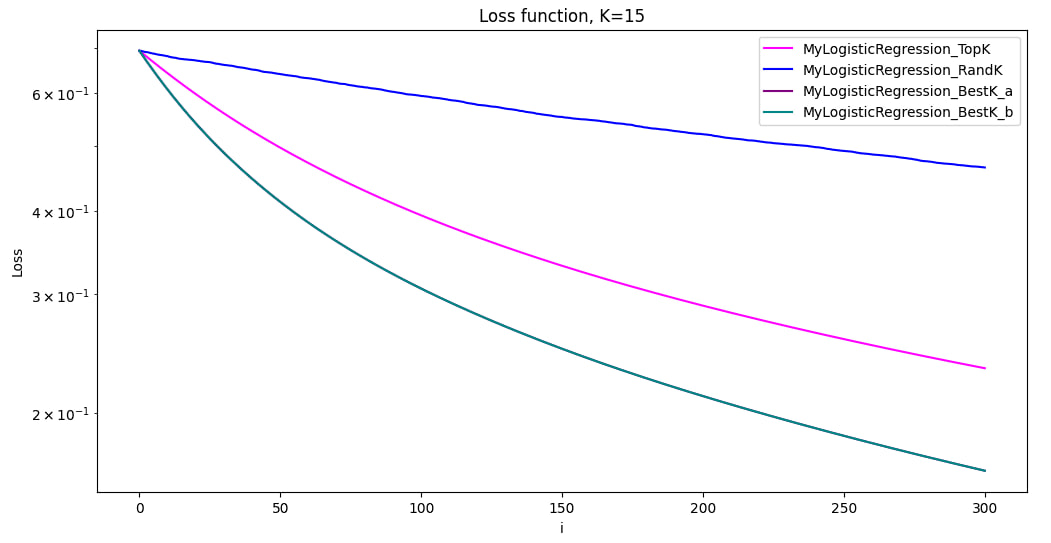
\includegraphics[width=1\linewidth]{1.jpg}}
\subcaptionbox{Зависимость нормы градиента от итерации}
  {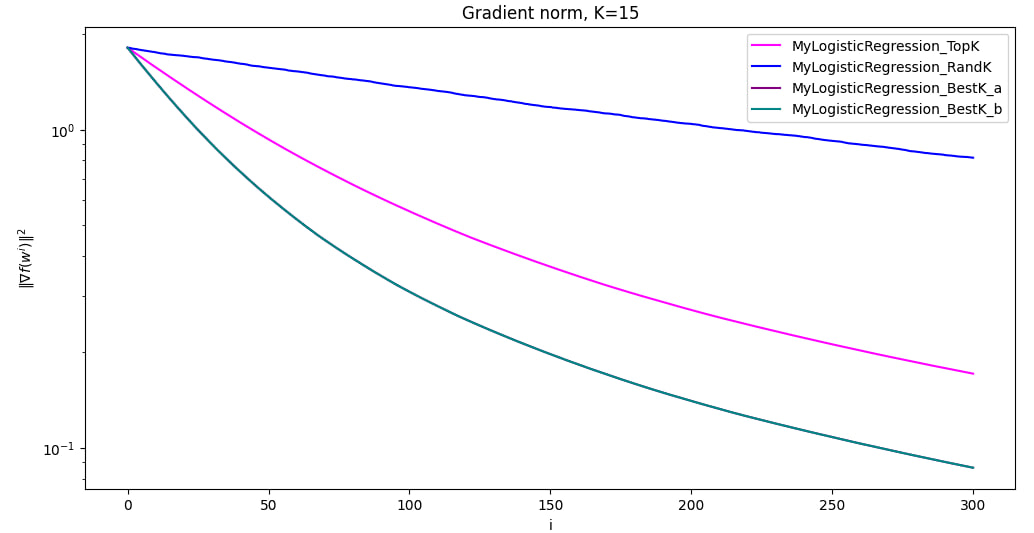
\includegraphics[width=1\linewidth]{2.jpg}}
\label{exper1_main}
\end{figure}

Теперь будем обучать нейросеть для датасета mushrooms. Получаем следующие результаты :
\begin{figure}[H]
\centering
\subcaptionbox{Зависимость функции потерь от эпохи}
  {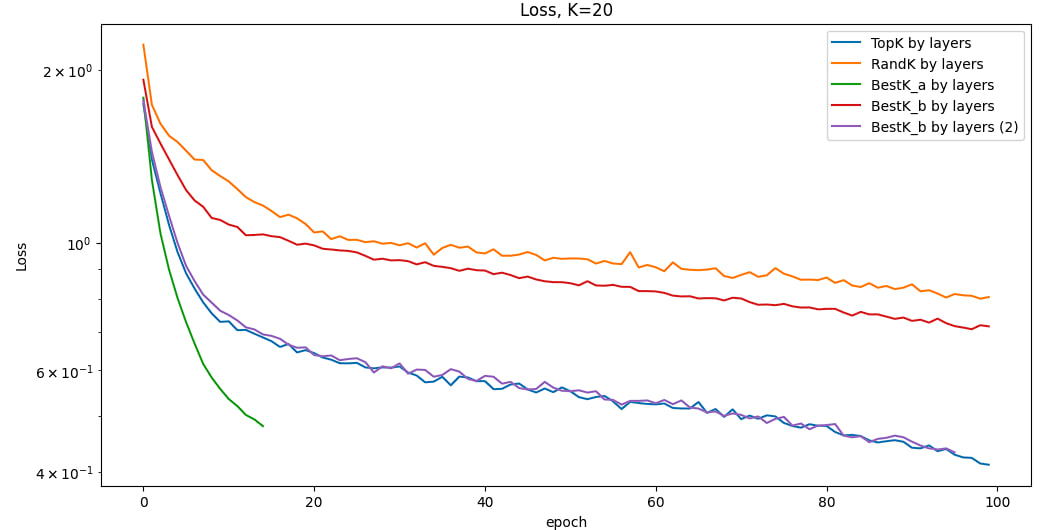
\includegraphics[width=1\linewidth]{3.jpg}}
\subcaptionbox{Зависимость точности от эпохи}
  {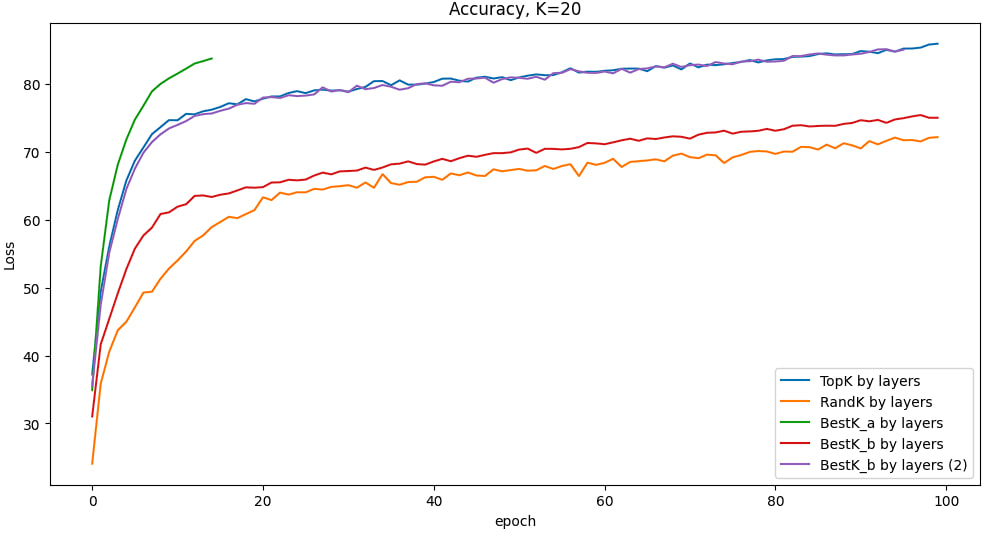
\includegraphics[width=1\linewidth]{4.jpg}}
\label{exper1_main}
\end{figure}

Хочу обратить внимание на реальное время для обучения :
\begin{figure}[H]
\centering
\subcaptionbox{Зависимость функции потерь от времени обучения}
  {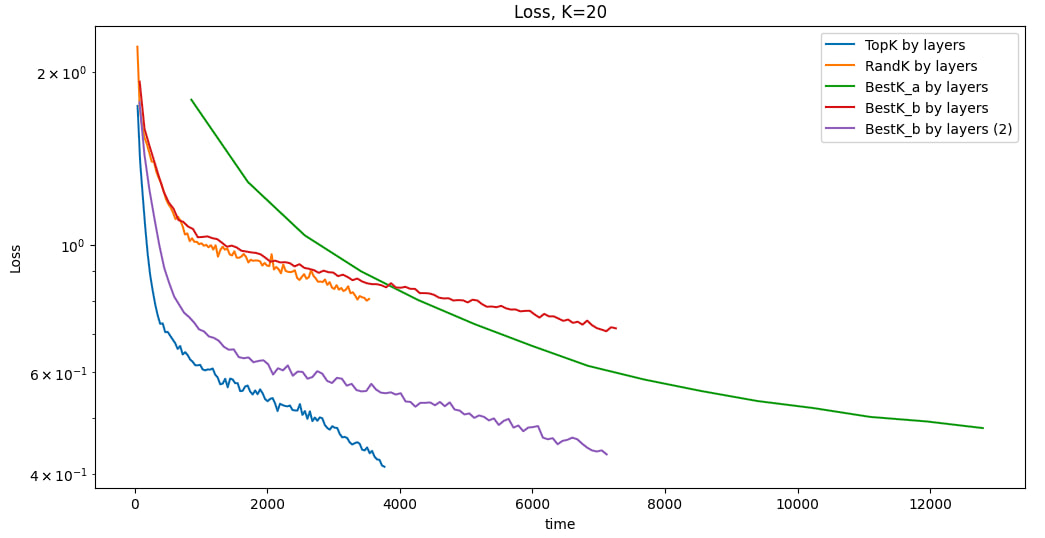
\includegraphics[width=1\linewidth]{5.jpg}}
\subcaptionbox{Зависимость точности от времени}
  {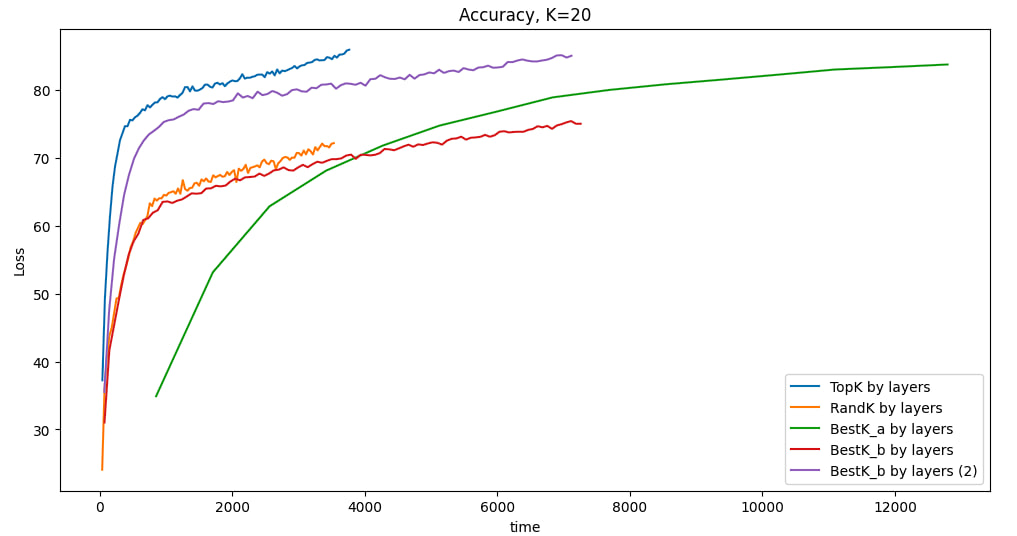
\includegraphics[width=1\linewidth]{6.jpg}}
\label{exper1_main}
\end{figure}

\subsection{Анализ полученных результатов}
Можно сделать следующие выводы относительно результатов эксперимента
\begin{enumerate}
    \item Методы действительно сходятся.
    \item Методы показывают скорость сходимости более высокую, чем $Rand_k$, что согласуется с теорией.
    \item Имеет место более высокая скорость сходимости методов (а), (b) и (c) в некоторых задачах. Однако они обходят вычислительно дороже, чем стандартные. 
\end{enumerate}

\section{Итог}
\begin{enumerate}
    \item Предложены и опробованы 3 новых оператора сжатия
    \item Получены гарантии сходимости этих методов
    \item Показано превосходство новых методов над стандартными.
\end{enumerate}


\bibliographystyle{unsrt}
\bibliography{bibliography}
\end{document}